%%%%%%%%%%%%%%%%%%%%%%%%%%%%%%%%%%%%%%%%%
% baposter Portrait Poster
% LaTeX Template
% Version 1.0 (15/5/13)
%
% Created by:
% Brian Amberg (baposter@brian-amberg.de)
%
% This template has been downloaded from:
% http://www.LaTeXTemplates.com
%
% License:
% CC BY-NC-SA 3.0 (http://creativecommons.org/licenses/by-nc-sa/3.0/)
%
%%%%%%%%%%%%%%%%%%%%%%%%%%%%%%%%%%%%%%%%%

%----------------------------------------------------------------------------------------
%	PACKAGES AND OTHER DOCUMENT CONFIGURATIONS
%----------------------------------------------------------------------------------------

\documentclass[a0paper,portrait]{baposter}

\usepackage[font=small,labelfont=bf]{caption} % Required for specifying captions to tables and figures
\usepackage{booktabs} % Horizontal rules in tables
%\usepackage{cite} % Makes references in series go [2,5,8-12] 
\usepackage[utf8]{inputenc}
\usepackage{pbox}
\usepackage{enumitem}
\usepackage{ragged2e}
\usepackage{caption}
\usepackage{graphicx}
\captionsetup{justification=raggedright,singlelinecheck=false}
\newcommand{\degree}{\ensuremath{^\circ}}
\graphicspath{{Images/}} % Directory in which figures are stored

%\usepackage[backend=biber,style=ieee,]{biblatex}
%\addbibresource{references.bib}

\definecolor{bordercol}{RGB}{200,200,200} % Border color of content boxes
\definecolor{headercol1}{RGB}{135, 206, 235} % Background color for the header in the content boxes (left side)
\definecolor{headercol2}{RGB}{0, 10, 255} % Background color for the header in the content boxes (right side)
\definecolor{headerfontcol}{RGB}{255, 255, 255} % Text color for the header text in the content boxes
\definecolor{boxcolor}{RGB}{255, 255, 255} %Background color for the content in the content boxes
\definecolor{backgroundcol}{RGB}{255, 255, 255} % Background color for the whole poster. For image as background, see below
%\definecolor{backgroundcol}{RGB}{000, 000, 000} % Background color for the whole poster. For image as background, see below

%% For colours that can be used for NTNU posters, see https://innsida.ntnu.no/logo-og-maler 

\begin{document}

%% IMAGE AS BACKGROUND
%\background{ % Set the background to an image (background.pdf)
%\begin{tikzpicture}[remember picture,overlay]
%\draw (current page.north west)+(-2em,2em) node[anchor=north west]
%{\includegraphics[height=1.1\textheight]{background.pdf}};
%\end{tikzpicture}
%}

\begin{poster}{grid=false,eyecatcher=false,borderColor=bordercol,headerColorOne=headercol1,headerColorTwo=headercol2,headerFontColor=headerfontcol,boxColorOne=boxcolor,headershape=roundedright,headerfont=\Large\sf\bfseries,textborder=rectangle,bgColorOne=backgroundcol,bgColorTwo=backgroundcol,background=plain,headerborder=open,boxshade=plain}
{} % Eye catcher (empty)
{\centering\vspace*{0.0em}\sf\bf ClaimGuard: A Blockchain-Backed Access Control
Gateway for Privacy-Preservation in Auto-Insurance
Claims} % Poster title
{\centering \vspace{0.2em} \scriptsize Anthony Uchenna Eneh, Love Allen Chijioke Ahakonye, Jae Min Lee, Dong-Seong Kim \\
\vspace{0.2em} \tiny Networked Systems Laboratory, Department of IT Convergence Engineering \\
} % Author addresses
{\centering\vspace{0.2em} Kumoh National Institute of Technology, Gumi 39177, South Korea
}
%
%----------------------------------------------------------------------------------------
%	TITLE AND AUTHOR NAME
%----------------------------------------------------------------------------------------
%
%{\includegraphics[scale=0.3]{KICS_FALL_2022_PAPER NO..png}} %paperno
%{\includegraphics[scale=0.3]{ntnu.png}} %universitylogo

% \headerbox{Title{name=topic1,span=1,column=0,below=motivation,height=0.15}{
% PAPER No.: GWEQC-0377 
% }

\headerbox{Motivation}{name=background,column=0,row=0,height=0.24}{
\begin{itemize}
    \item Policy expressiveness: Claims workflows need case-, time-, and purpose-specific rules that cloud RBAC cannot represent.
    \item Cross-party accountability: Multi-organization evidence sharing lacks a unified, tamper-evident audit trail.
    \item Insider over-trust risk: Cloud operators and over-privileged roles can bypass intended controls without an on-chain decision path.
    \item Practical deployability: Existing blockchain ABAC work seldom bridges to legacy object stores

    \end{itemize}
}

\headerbox{Introduction}{name=topic1,span=2,column=1,row=0,height=0.1}{
Auto‑insurance claims increasingly depend on heterogeneous digital evidence shared across multiple organizations. Yet, prevailing cloud RBAC is coarse‑grained, weakly auditable, and poorly suited to case‑specific constraints. This paper presents ClaimGuard, a blockchain‑backed ABAC gateway that evaluates policies on‑chain and issues short‑lived capability tokens for controlled access to off‑chain evidence. Results show interactive performance and strong authorization correctness.
}


\headerbox{Contribution}{name=topic2,span=1,column=0,below=background,height=0.25}{
\begin{itemize}
    \item Gateway enforcement: Introduce a blockchain-backed ABAC gateway that mediates all evidence access instead of direct cloud RBAC.
    \item On-chain policy engine: Implement smart-contract ABAC rules and decision logging to provide fine-grained, tamper-evident authorization.
    \item Capability binding: Issue short-lived capability tokens tied to subject, resource, action, and expiry to constrain access at the storage layer.
    \item Practical validation: Demonstrate deployability with an end-to-end prototype and performance evaluation under realistic workloads.
\end{itemize}
}

\headerbox{Methodology}{name=topic3,span=2,column=1,below=topic1,height=0.39}{
\newsavebox{\methodtextbox}
\setbox\methodtextbox=\vbox{%
  \hsize=0.3\textwidth
  \noindent We model the claims workflow as subject, resource, and environment attributes and encode ABAC rules in Solidity contracts. A REST gateway receives access requests, queries on-chain checkAccess, and issues short-lived capability tokens bound to subject, resource, action, and expiry. Evidence access is granted only with valid tokens at the storage adapter. We deploy contracts on a local Ethereum network, seed subjects/resources, and run scripted load tests to measure latency, throughput, and policy-update costs. We log decisions on-chain for auditability analysis.
}
\noindent
\begin{minipage}[t]{0.3\textwidth}
  \vspace{0pt}%
  We model the claims workflow as subject, resource, and environment attributes and encode ABAC rules in Solidity contracts. A REST gateway receives access requests, queries on-chain checkAccess, and issues short-lived capability tokens bound to subject, resource, action, and expiry. Evidence access is granted only with valid tokens at the storage adapter. We deploy contracts on a local Ethereum network, seed subjects/resources, and run scripted load tests to measure latency, throughput, and policy-update costs. We log decisions on-chain for auditability analysis.
\end{minipage}
\hfill
\begin{minipage}[t]{0.7\textwidth}
  \vspace{0pt}%
  \centering
  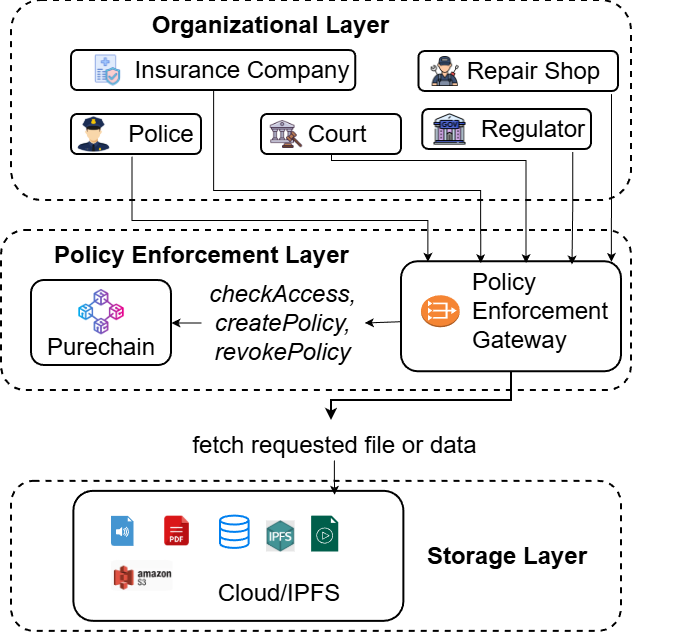
\includegraphics[height=\dimexpr\ht\methodtextbox+\dp\methodtextbox\relax]{figures/architecture.png}
  \\
  \textit{Fig.1:  Claimguard Architecture}
\end{minipage}
}

 

\headerbox{Performance Evaluation}{name=results,span=3,column=0,below=topic2,height=0.27}{
\centering
\begin{minipage}[t]{0.5\textwidth}
    \centering
    
\includegraphics[width=\linewidth]{figures/throughput.png}
   % \begin{center} 
    %\textit{Fig.2:  Confusion Matrix}
  %\end{center}
\end{minipage}
\hfill
\begin{minipage}[t]{0.5\textwidth}
    \centering
    
\includegraphics[width=\linewidth]{figures/latency_bar_chart.png}
   % \captionof{figure}{Fig. 3: (add caption here)}
    \label{fig:roc_or_whatever}
\end{minipage}
% \hfill
% \begin{minipage}[t]{0.3\textwidth}
%     \centering
%     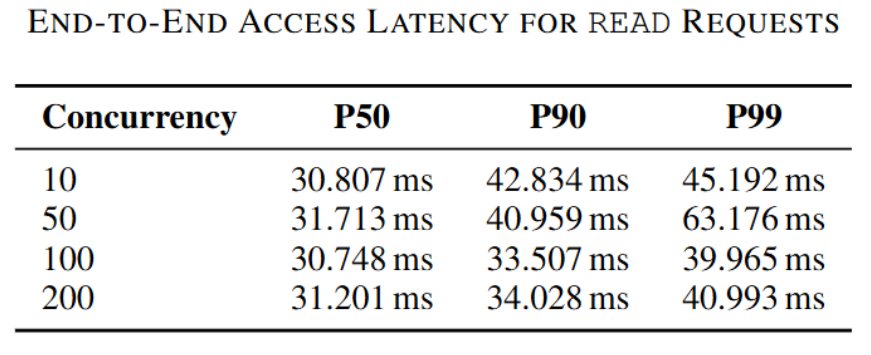
\includegraphics[width=\linewidth]{figures/end_to_end_latency.png}
%    % \captionof{figure}{Fig. 3: (add caption here)}
%     \label{fig:roc_or_whatever}
% \end{minipage}
}




\headerbox{Conclusion \& Future Work}
{name=conclusion,span=2,column=0,below=results,above=bottom, height=0.1}{
Results show that ClaimGuard sustains interactive access latency, high throughput, and fast policy updates while producing zero false accepts, indicating correct enforcement of on‑chain ABAC decisions. These findings support the conclusion that a blockchain‑backed gateway can deliver fine‑grained, auditable access control without prohibitive overhead for multi‑party claims workflows. Future work will broaden evaluation by comparing against cloud‑only RBAC baselines, testing under realistic network conditions and consortium deployments, and using real claims datasets. We also plan to explore cross‑chain interoperability and privacy‑preserving attribute encoding while keeping ML‑based risk scoring outside the current scope. \\
{
\includegraphics[scale=0.6]{assets/KIT_1 (1).png}} %universitylogo
{
\includegraphics[scale=0.6]{assets/NSL_LAB.png}} %universitylogo
%{\includegraphics[scale=0.8]{ICT_RESEARCH CENTRE.png}}
%{\includegraphics[scale=0.4]{KICS_LOGO.png}}
{
\includegraphics[scale=0.3]{assets/KIT.png}}
}


\headerbox{Acknowledgement}{name=references,column=2,below=results,above=bottom, height=0.1}{This work was partly supported by Innovative Human
Resource Development for Local Intellectualization program
through the IITP grant funded by the Korea government
(MSIT) (IITP-2025-RS-2020-II201612, 25\%) and by Priority
Research Centers Program through the NRF funded by the
MEST (2018R1A6A1A03024003, 25\%) and by the MSIT,
Korea, under the ITRC support program (IITP-2025-RS-2024-
00438430, 25\%) and by Basic Science Research Program
through the National Research Foundation of Korea(NRF)
funded by the Ministry of Education(RS-2025-25431637,
25\%).

\scriptsize %\tiny%small % Reduce the font size in this block
\renewcommand{\section}[2]{\vskip 0.05em} % Get rid of the default "References" section title
%\bibliographystyle{unsrt}

%\printbibliography
}

\end{poster}
\end{document}